\documentclass[12pt,a4paper]{article}
\usepackage[utf8]{inputenc}
\usepackage{amsmath}
\usepackage{amsfonts}
\usepackage{amssymb}
\usepackage{graphicx}
\usepackage{polski}
\usepackage{mathtools}
\usepackage[T1]{fontenc}
\usepackage{pdflscape}
\usepackage{graphicx}
\usepackage{caption}
\usepackage{subcaption}
\usepackage{floatrow}
\usepackage{float}
\DeclarePairedDelimiter{\ceil}{\lceil}{\rceil}

\title{Rozmieszczanie kamer bezpieczeństwa}
\author{Przemysław Kopański \\ Mateusz Forc}

\begin{document}
\maketitle
\tableofcontents
\section{Treść zadania}
Jak optymalnie rozmieścić kamery monitoringu w ustalonym pomieszczeniu (rzut z góry),
aby minimalną liczbą kamer móc obserwować dowolne miejsce 
(z uwzględnieniem maksymalnej dopuszczalnej odległości od kamery).
%
\newpage
\section{Przyjęte założenia}
\begin{itemize}
\item wszystkie kamery są takie same (mają taki sam zasięg)
	\begin{itemize}
	\item zasięg kamery jest kołem o stałym promieniu
	\item promień zasięgu kameru wynosi 2 (możliwa interpretacja - średnica kamery wynosi 4 metry)
	\end{itemize}
\item rzut pomieszczenia reprezentowany jest przez zbiór punktów
	\begin{itemize}
	\item punkty mają współrzędne odpowiadające I ćwiartce wykresu \[x \geq 0, y \geq 0\]
	\item punkty podawane są jako lista, która reprezentuje zamknięty wielokąt - muszą one zostać
	      podane we właściwej kolejności, tak aby można je było jednoznacznie połączyć 
	      (każde dwa kolejne punkty łączone są w odcinek)
	\end{itemize}
\end{itemize}
%
\section{Przestrzeń przeszukiwań}
Pojedynczym elementem przestrzeni przeszukiwań jest zbiór kamer wraz z ich pozycjami. \\
Rozwiązanie początkowe zawiera zbiór składający się z $\lceil$obszar rzutu/obszar jednej kamery$\rceil$ kamer
rozmieszczonych losowo wewnątrz wielokątu.
Do kolejnego stanu możemy przejść poprzez dodanie/usunięcie kamery lub przemieszczenie
jednej z aktualnie umieszczonych kamer.
Do zbioru kamer nie można wstawić kamery, która jest na zewnątrz obserwowanego pomieszczenia.
%
\newpage
\section{Funkcja celu}
Dostępna informacja: \\
\footnotesize
$k_{min}$ - minimalna teoretyczna liczba kamer dla aktualnie rozpatrywanego rzutu \\ \indent ($\lceil$obszar rzutu/obszar jednej kamery$\rceil$) \\
\normalsize
%
\newline
Parametry zadania: \\
$d_k$ - koszt użycia kamery \\
$d_p$ - wartość pokrycia 1\% powierzchni\\
\newline
Funkcja:
$f(p, k) = d_p*p - \frac{100d_k}{k_{min}}*max(0,k - k_{min}) $ \\ \\
gdzie: \\
p - \% pokrycia dla danego stanu \\
k - ilość użytych kamer w danym stanie \\ \\
Zadanie polega na maksymalizacji funkcji f. \\ \\ 
Przykładowo \\
$ d_p = 1$ \\
$ d_k = 1$ \\ \\ 
Dla podanych parametrów algorytm będzie znajdował ,,złoty środek pomiędzy'' 
procentem pokrycia a ilością użytych kamer.
Odpowiednio przeskalowując podane parametry i trzymajac odpowiedni 
stosunek pomiędzy tymi wartościami,
mozemy sterowac na czym bardziej nam zależy, jeżeli np 
$d_p = 2d_k = 1 $ to będziemy w stanie zaakceptować dwukrotna 
ilość kamer w zamian za dwukrotnie większe pokrycie.
%
\subsection{Przykład}
\begin{center}
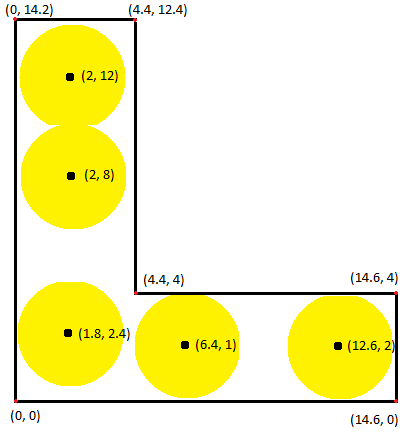
\includegraphics[scale=0.9]{example_projection.png}
\end{center}
Podane pomieszczenie ma pole powierzchni równe 103.38. \\
Zasięgi kamer są między sobą rozłączne, a ich pole wynosi 62.83. \\
Minimalna teoretyczna liczba kamery wynosi 9. \\
Pokrycie dla danego stanu wynosi 60.8\%. \\ \\
Dla parametrów:
$d_p = 1 d_k = 1$ \\
wartość funkcji wynosi 60.8-0 = 60.8 \\ \\
Podane rozwiązanie posiada zbyt małą liczbę kamer, by móc w stanie pokryć całą powierzchnię.
\section{Metaheurystyka}
Zastosowany zostanie stabuizowany algorytm symulowanego wyżarzania.
Ze względu na to, że stworzenie funkcji heurystycznej do badanej przestrzeni jest obliczalnie
trudne, użycie metody A* jest niewskazane.
Algorytmy wspinaczkowe nie sprawdzą się w opisywanej przestrzeni ze względu na dużą liczbę
ekstremów lokalnych. Stosując algorytm symulowanego wyżarzania zapewnione jest,
że algorytm nie ‘utknie’ w ekstremum. Wraz z rosnącą liczbą iteracji można zmniejszać temperaturę,
w celu znalezienia coraz lepszego rozwiązania. Dodatkowym mechanizmem pozwalającym uniknąć
zakotwiczenia w ekstremum lokalnym jest tabuizacja.\\

Podana metoda wymaga strojenia ze względu na 2 parametry:
\begin{enumerate}
  \item wielkość kolejki tabu - określa ile maksymalnie jednocześnie punktów przestrzeni może ulec tabuizacji
  \item parametr funkcji temperatury - do doboru temperatury zostanie wykorzystana funkcja zależna od numeru iteracji, która udostępni parametr do strojenia
\end{enumerate}

\section{Przewidywane wyniki pracy}
Dla kilkunastu zadanych rzutów ilustrujących różne warianty pomieszczeń np. długie, wąskie i kręte,
duże otwarte zostaną przeprowadzone symulacje w celu odnalezienia i zaprezentowania
parametrów funkcji celu, które pozwalają implementacji na znalezienie możliwie
najlepszego rozwiązania dla danego rodzaju przypadku. \\ \\
Wyniki zostaną zaprezentowane jako zestawy rzutów oraz wykresów
ilustrujących pokrycie w zależności od parametrów: $d_p$ i $d_k$ wraz z wyróżnionym zestawem
parametrów dla każdego zestawu, który ilustruje najlepsze rezultaty.

\newpage
\section{Podsumowanie}
Dla różnych rodzajów rzutów, uruchomiony został zaimplementowany algorytm, wraz z różnymi parametrami $d_p$, $d_k$ oraz wielkością kolejki tabu.

\subsection{Przykłady testowe}
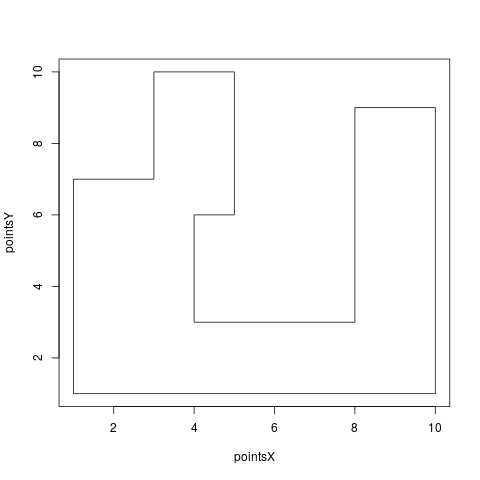
\includegraphics[scale=0.4]{mediumMap.png} 
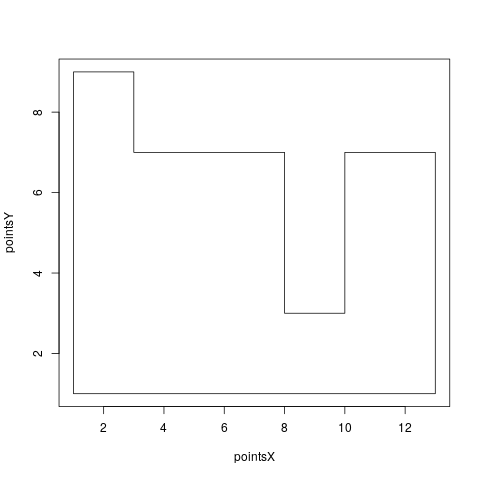
\includegraphics[scale=0.4]{mediumMap2.png} \\
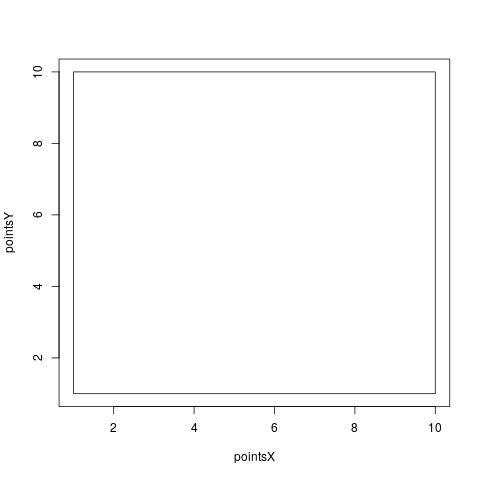
\includegraphics[scale=0.4]{openSpace.png}
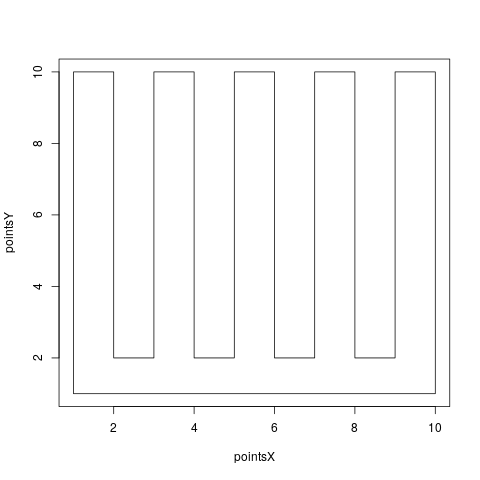
\includegraphics[scale=0.4]{slimLines.png} \\
Przetestowane zostały powyższe mapy w różnych skalach. Znajdują się tutaj dwa przypadki skrajne jeżeli chodzi o szerokość i pojedyńczego korytarza na rzucie jak i o ilość korytarzy oraz dwa przypadki dosyć wyważone. \\
W każdym przypadku promień kamery wynosił 2 i w przypadku skalowania był odpowiednio powiększany.

\begin{landscape}
\pagestyle{empty}
\begin{figure}
\begin{floatrow}
       \ffigbox[\FBwidth]{\caption{MediumMap, $d_p=1$, $d_k=0.1$, $skala=2$}\label{fig-3}}{%
         \includegraphics[width=0.5\textwidth]{{mediumMap_1_0.1_2}.png}
       }
       \ffigbox[\FBwidth]{\caption{MediumMap, $d_p=1$, $d_k=0.1$, $skala=5$}\label{fig-4}}{%
         \includegraphics[width=0.5\textwidth]{{mediumMap_1_0.1_5}.png}
       }
       \end{floatrow}
\end{figure}
\end{landscape}

Podane wykresy prezentuja przykładowe działanie algorytmu dla podanych parametrów.
Pierwszy wykres pokazuje aktualnie wybrany punkt w jednej iteracji projektu.
Drugi wykres prezentuje punkt sąsiedni wygenerowany w danej iteracji algorytmu.
Może on zostać wybrany przez algorytm jako następny punkt.
Trzeci wykres prezentuje wszystkie wygenerowane rozwiązania przez algorytm, ze względu
na ilość użytych kamer oraz procentu pokrycia powierzchni przez kamery.

\subsection{Wnioski}
Na podstawie przeprowadzonych symulacji nie zauważyliśmy znaczącej różnicy w pracy dla różnej wartości wielkości kolejki.
\begin{figure}[h]
\begin{floatrow}
       \ffigbox[\FBwidth]{\caption{MediumMap, $d_p=1$, $d_k=1$, $skala=5$, $queueSize=10$}\label{fig-5}}{%
         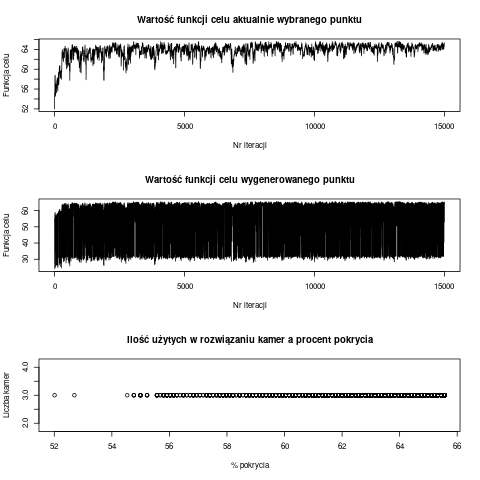
\includegraphics[width=0.5\textwidth]{queue10.png}
       }
       \ffigbox[\FBwidth]{\caption{MediumMap, $d_p=1$, $d_k=1$, $skala=5$, $queueSize=100$}\label{fig-6}}{%
         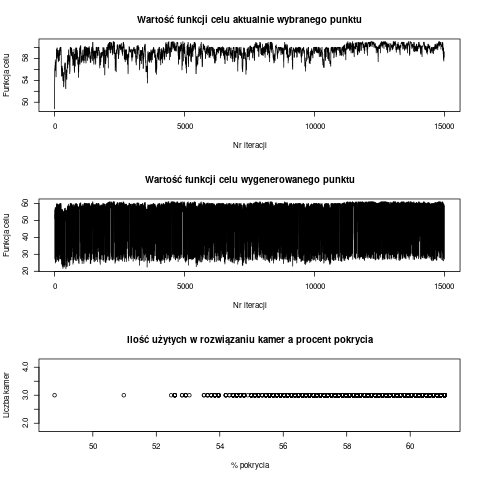
\includegraphics[width=0.5\textwidth]{queue100.png}
       }
       \end{floatrow}
\end{figure}

\newpage
\subsubsection{Wpływ parametrów $d_p$ i $d_k$ na zachowanie algorytmu}
\begin{figure}[h]
\begin{floatrow}
       \ffigbox[\FBwidth]{\caption{OpenSpace, $d_p=0.1$, $d_k=0.1$, $skala=5$}\label{fig-7}}{%
         \includegraphics[width=0.5\textwidth]{{openSpace_0.1_0.1_5}.png}
       }
       \ffigbox[\FBwidth]{\caption{MediumMap, $d_p=0.2$, $d_k=0.2$, $skala=5$}\label{fig-8}}{%
         \includegraphics[width=0.5\textwidth]{{mediumMap_0.2_0.2_5}.png}
       }
       \end{floatrow}
\end{figure}

Dla bardzo małych wartości $d_p$ i $d_k$ odnotowaliśmy zachowanie bardzo zbliżone do błądzenia przypadkowaego.
Wynika to z faktu, iż różnica pomiędzy kolejnymi rozwiązaniami jest niewielka, przez co istnieje duże prawdopodobieństwo wybrania punktu gorszego. Prawdopodobieństwo wybrania gorszego punktu wynosi
$exp(\frac{-|q(x)-q(y)|}{t})$, gdzie $q(x), q(y)$ to wartości funkcji celu dla punktu bazowego i jego wygenerowanego sąsiada, a $t$ - aktualna temperatura. W przypadku niższych wartości $d_p$ i $d_k$, podana funkcja dla danego $t$ osiąga
wartości bliskie jedności.
\begin{figure}[H]
\begin{floatrow}
       \ffigbox[\FBwidth]{\caption{MediumMap, $d_p=0.9$, $d_k=0.1$, $skala=5$}\label{fig-9}}{%
         \includegraphics[width=0.5\textwidth]{{mediumMap_0.1_0.1_5}.png}
       }
       \ffigbox[\FBwidth]{\caption{SlimMap, $d_p=1$, $d_k=0.1$, $skala=5$}\label{fig-10}}{%
         \includegraphics[width=0.5\textwidth]{{slimMap_1_0.1_5}.png}
       }
       \end{floatrow}
\end{figure}
Dla $d_p >> d_k$ dało sie zaobserwować częste dokładanie kamer. Wynika to z faktu, że koszt dodania kamery jest bardzo mały (róznica wartości funkcji celu) a prawdopodobieństwo dodania nowej kamery jest dosyć duże.

\begin{figure}[H]
\begin{floatrow}
       \ffigbox[\FBwidth]{\caption{MediumMap2, $d_p=1.0$, $d_k=0.7$, $skala=5$}\label{fig-11}}{%
         \includegraphics[width=0.5\textwidth]{{mediumMap2_1_0.7_5}.png}
       }
       \ffigbox[\FBwidth]{\caption{SlimMap, $d_p=1$, $d_k=0.4$, $skala=5$}\label{fig-12}}{%
         \includegraphics[width=0.5\textwidth]{{slimMap_1_0.4_5}.png}
       }
       \end{floatrow}
\end{figure}
Dla nierównomiernych powierzchni idealne wartości parametrów oscylują pomiędzy $dp=1, d_k\in \langle 0.4, 0.7 \rangle $.
Dzięki temu, gdy kolejne wygenerowane rozwiązanie będzie zawierało dodatkową kamerę, istnieje większa szansa,
że zostanie wybrane pomimo, że ta dodatkowa kamera mogłaby sie znajdować w nieoptymalnym dla niej miejscu w danej chwili.
W przypadku mapy zawierającej większą ilość wąskich korytarzy preferewana jest niższa wartość parametru $d_k$.


\newpage
\subsubsection{Zmiana interfejsu użytkownia}
Po przebadaniu zachowania algorytmu można zauważyć, że lepszym sposobem do strojenia algorytmu jest podanie
wspóczynnika $\frac{d_p}{d_k}$ zamiast poszczególnych wartości. Zapewniamy przez to uniknięcie nieintuicyjnej
różnicy zachowań algorytmu jak w przypadku uruchomieniu z argumentami $d_p=1, d_k=1$ a np. $d_p=0.5, d_k=0.5$.

\subsubsection{Zmiana reprezentacji problemu}
W dalekiej fazie prac nad projektem, doszliśmy do wniosku, że jednym z czynników, które spowalniają przebieg symulacji jest nieoptymalna reprezentacja problemu.\\
Lepszy pomysł reprezentacji: \\
Do każdego pola wewnątrz rzutu, przypisujemy liczbę całkowitą i rozwiązanie reprezentujemy jako zbiór owych liczb. \\
Dzięki takiemu podejściu, jestesmy w stanie pominąć kosztowne sprawdzanie poprawności punktów oznaczonych jako leżące w zasięgu kamer, które staraliśmy się optymalizować w trakcie prac nad implementacją.


\end{document}
